% !TEX root = ../Thesis.tex
% !TEX output_directory
\documentclass[11pt,a4paper,english,greek,twoside]{../Thesis}
\usepackage{subfig}
\usepackage{subcaption} 
\begin{document}
\chapter{Ηλεκτροεγκεφαλογραφία}
\section{Βιοηλεκτρικά Σήματα και Ηλεκτροεγκεφαλογράφημα}
%Στο εισαγωγικό κεφάλαιο εστιάσαμε στην σημασία της μελέτης του εγκεφάλου και των σημάτων που μπορούμε να εξάγουμε από αυτόν.
Τα βιοηλεκτρικά σήματα είναι το αποτέλεσμα των ηλεκτροχημικών μεταβολών που λαμβάνουν χώρα εντός και μεταξύ των κυττάρων των νεύρων καθώς και των μυών. Πιο συγκεκριμένα, εάν ένα τέτοιο κύτταρο δεχθεί ερέθισμα ισχυρότερο από ένα κατώφλι συνήθως μεταξύ  -55mV και -50mV, τότε θα παράγει ένα δυναμικό δράσης το οποίο θα μεταδοθεί και θα διεγείρει γειτονικά κύτταρα. Αυτή η ομαδική δραστηριότητα των κυττάρων παράγει ηλεκτρικά πεδία ικανά να ανιχνευτούν με την βοήθεια ηλεκτροδίων τα οποία τοποθετούνται στην επιφάνεια του αντίστοιχου οργάνου, είτε στην δερματική επιφάνεια πάνω αυτό το όργανο. Όταν το ζωτικό αυτό όργανο είναι ο εγκέφαλος τότε το βιοηλεκτρικό σήμα ονομάζεται Ηλεκτροεγκεφαλογράφημα (ΗΕΓ – EEG) και η πρώτη καταγραφή ΗΕΓ, έγινε το 1924 από τον Γερμανό ψυχίατρο Hans Berger. 

Η Ηλεκτροεγκεφαλογραφία, είναι η πρώτη μέθοδος που χρησιμοποιήθηκε για την απεικόνιση της εγκεφαλικής δραστηριότητας, πριν την εμφάνιση μεθόδων όπως η μαγνητική τομογραφία (MRI) και τομογραφία εκπομπής ποζιτρονίων (PET). Παρουσιάζει σημαντικά πλεονεκτήματα όπως το ότι είναι πολύ οικονομικά προσιτή μέθοδος, συγκρινόμενη με τις άλλες που αναφέρθηκαν, και το γεγονός πως έχει πολύ χρονική ανάλυση (temporal resolution), καθώς ενώ οι μεταβολές δυναμικού του εγκεφάλου συμβαίνουν σε πολύ μικρά χρονικά διαστήματα, οι εγκεφαλογράφοι πλέον κάνουν δειγματοληψία του σήματος με συχνότητες έως και $2048Hz$, διατηρώντας σχεδόν όλη την πληροφορία του σήματος. Ωστόσο, όσον αφορά την χωρική ανάλυση (spatial resolution), ισχύει κάτι αντίστοιχο. Τα ηλεκτρικά σήματα από την στιγμή που ξεκινάνε από την πηγή τους, μέχρι να καταλήξουν στα ηλεκτρόδια, διασκορπίζονται κατά την διέλευση τους από το κρανίο. Συνεπώς το σήμα που ανιχνεύεται από ένα ηλεκτρόδιο σε μια συγκεκριμένη περιοχή δεν προέρχεται μόνο από το σημείο του εγκεφάλου που καλύπτει, αλλά και από τα γειτονικά. Αυτό το πρόβλημα μπορεί να αντιμετωπιστεί κάνοντας χρήση περισσότερων ηλεκτροδίων, και χρήσης τεχνικών χωρικού φιλτραρίσματος, για την λύση του αντίστροφου προβλήματος, δηλαδή την εύρεση του πραγματικού ηλεκτρικού σήματος που ξεκίνησε από κάθε περιοχή του εγκεφάλου. Ένας άλλος τρόπος είναι να χρησιμοποιηθούν ηλεκτρόδια που εισχωρούν σε μεγαλύτερο βάθος, πλησιάζοντας την πηγή του σήματος, πριν αυτό αλλοιωθεί από το κρανίο, προσφέροντας πολύ καλύτερη χωρική ανάλυση. Το εγκεφαλογράφημα που κάνει χρήση τέτοιου τύπου ηλεκτρόδια, ονομάζεται επεμβάτικο (invasive EEG).
\section{Εγκεφαλογράφος}
Η συσκευή που χρησιμοποιείται για την καταγραφή του εγκεφαλογραφήματος, ονομάζεται εγκεφαλογράφος, και είναι μια πολύπλοκη συσκευή με διάφορα υποσυστήματα. Από τις αρχές του 20ου αιώνα που δημιουργήθηκε ο πρώτος εγκεφαλογράφος, μέχρι σήμερα, έχουν υπάρξει δραματικές αλλαγές στον τρόπο υλοποίησης τους, με ποιο σημαντική την εισαγωγή της ψηφιακής τεχνολογίας στην αλυσίδα επεξεργασίας του σήματος. Τα υποσυστήματα που παραθέτονται στην συνέχεια, περιέχονται σε όλους τους σύγχρονους εγκεφαλογράφους, χωρίς να σημαίνει πως δεν υπάρχουν παραλλαγές και επιπλέον υποσυστήματα σε άλλους.

\subsection{Ηλεκτρόδια}
  Tα ηλεκτρόδια στην πραγματικότητα, είναι μετατροπείς, οι οποίοι ανιχνεύουν την κατανομή των ιόντων στην επιφάνεια των ιστών που καλύπτουν, μετατρέποντας το ιοντικό ρεύμα σε ρεύμα ηλεκτρόνιων. Τα ηλεκτρόδια χωρίζονται σε δύο βασικές κατηγορίες, τα 'υγρά' (wet) και τα 'στεγνά' (dry) και καθένα από αυτά μπορεί να είναι είτε μιας χρήσης, είτε επαναχρησιμοποιούμενο. 
\begin{itemize}
    \item{Υγρά (Wet) Ηλεκτρόδια}
    \par Σε αυτόν τον τύπο, χρησιμοποιείται αγώγιμο υγρό μεταξύ του δέρματος και του ηλεκτροδίου προκειμένου να επιτευχθεί αντίσταση επαφής περίπου $5kΩ$ \cite{}, έτσι ώστε να εξασφαλιστεί καλή ποιότητα σήματος ΗΕΓ με υψηλό λόγο σήματος προς θόρυβο (SNR). Ο συχνότερος τύπος ‘υγρών’ ηλεκτροδίων είναι τα αργύρου-χλωριούχου αργύρου (Ag – AgCL), τα οποία αποτελούνται απο ένα δισκίο, από καθαρό άργυρο $99.9\% $, επικαλυμένα από ένα λεπτό στρώμα χλωριούχου αργύρου. Είναι ευρέως χρησιμοποιούμενα λόγω του χαμηλού κόστους τους, της ευκολίας στην χρήση τους, καθώς και το ότι δεν είναι τοξικά. σε μορφή δισκίων η κυπέλλων \textcolor{red}{(βαλε εικονα)}.  
    \par Ένα άλλο είδος υγρών ηλεκτροδίων, χρησιμοποιούνται στον εγκεφαλογράφο Epoc που κατασκευάζεται από την εταιρεία Emotiv, και αποτελούνται από ένα χάλκινο ηλεκτρόδιο, επικαλυμμένο από μια λεπτή στρώση χρυσού. Η επαφή με το δέρμα γίνεται μέσω ενός κυλινδρικού σφουγγαριού (felt pad), το οποίο διαποτίζετε σε αλατούχο διάλυμα (saline) για την ελάττωση της αντίστασης επαφής.
    \par Παρότι η επίδοση των υγρών ηλεκτροδίων είναι πολύ ικανοποιητική, και χρησιμοποιείται ως σημείο αναφοράς για τις νέες τεχνολογίες ηλεκτροδίων που εμφανίζονται, μια σειρά απο μειονεκτήματα, εμποδίζει την χρήση τους σε περιβάλλοντα εκτός εργαστηρίου. Το πρώτο και βασικότερο είναι η δυσκολία που έχουν στην εφαρμογή τους και η άβολη αίσθηση που έχουν κατά την χρήση τους λόγω του υγρού στοιχείου. Συνήθως, απαιτείται ειδικός καθαρισμός  του σημείου επαφής πριν την χρήση, για την επίτευξη καλύτερου σήματος, αλλά και μετά το πέρας της διαδικασίας, για να καθαριστεί το δέρμα από  τα υπολείμματα του αγώγιμου υγρού. Επιπλέον, η επίτευξη της επιθυμητής αντίστασης που αναφέρθηκε προηγουμένως, μπορεί να καθυστερήσει σημαντικά. Τέλος, λόγω της πτητικότητας του αγώγιμου υγρού, υπάρχει ένα μικρό περιθώριο λίγων ωρών, πριν να ξαναχρειαστεί να το ανανεώσουμε.
    
    \item{Στεγνά (Dry) Ηλεκτρόδια}
    \par Τα προηγούμενα μειονεκτήματα έρχεται να τα καλύψει μια νέα τεχνολογία ηλεκτροδίων που δεν χρησιμοποιούν κάποιο αγώγιμο υγρό, αλλά εκμεταλλεύομενα τις εξελίξεις στον τομέα τεχνολογίας υλικών και των μικρο-συστημάτων (MEMS), προσπαθούν να επιτύχουν ποιότητα σήματος συγκρίσιμη με αυτή των υγρών ηλεκτροδίων. Λόγω της έλειψης αγώγιμου υγρού, η αντίσταση επαφής μεταξύ των ηλεκτροδίων και του δέρματος είναι πολύ μεγαλύτερη σε σχέση με τα υγρά ηλεκτρόδια, συνεπώς περιέχουν και έναν χαμηλής ενέργειας ενισχυτή οργανολογίας (instrumental amplifier) με πολύ υψηλή αντίσταση εισόδου, προκειμένου να υπάρχει όσο το δυνατόν μικρότερη απώλεια σήματος, και γι αυτό το λόγο αναφέρονται και στην βιβλιογραφία και ως ενεργά στεγνά ηλεκτρόδια (active dry electrodes). Υπάρχουν αρκετές κατηγορίες τέτοιων ηλεκτροδίων ανάλογα με την τεχνολογία κατασκευής τους και τον τρόπο επαφής τους με το δέρμα. Τα ακιδωτά ηλεκτρόδια αποτελούνται από μια συστοιχία ακίδων που είτε έρχεται σε επαφή με το δέρμα, είτε το τρυπάει για ελάχιστα μικρόμετρα, προκειμένου να διαπεράσει την εξωτερική του στρώση (stratum corneum), η οποία και ευθύνεται για το μεγαλύτερο ποσοστό της αντίστασης επαφής μεταξύ δέρματος και ηλεκτροδίου \cite{lopez2014dry}. Στη δημοσίευση \cite{sullivan2007low} χρησιμοποίησαν πυκνωτικά ηλεκτρόδια που δεν έρχονται σε επαφή με το δέρμα, προκειμένου να αποφύγουν αλλοίωση του σήματος με τα μαλλιά, αυξάνωντας όμως δραματικά την αντίσταση μεταξύ δέρματος και ηλεκτροδίου. Παρότι η έρευνα προς αυτή του του είδους τα ηλεκτρόδια φαίνεται ελπιδοφόρα και ικανή να αντιμετωπίσει τα προβήματα των υγρών ηλεκτροδίων, στην πλειοψηφία των δημοσιέυσεων είτε δεν αναφέρονται λεπτομέρειες σχετικά με την κατασκευή τους, είτε δεν γίνεται σύγκριση των αποτελεσμάτων με τις επιδόσεις των υγρών ηλεκτροδίων, συνεπώς υπάρχει ακόμα δρόμος προς αυτήν την κατεύθυνση \cite{lopez2014dry}.
    

\end{itemize}
\subsection{Ενίσχυση και Επεξεργασία Σημάτων}
  Τα σήματα που λαμβάνονται από τα ηλεκτρόδια στην επιφάνεια του δέρματος κυμαίνονται μεταξύ $10μV$ και $100μV$, και πρέπει να ενισχυθούν σημαντικά προκειμένου να γίνει η επεξεργασία τους στα επόμενα στάδια. Το στάδιο της ενίσχυσης περιλαμβάνει αρχικά έναν διαφορικό ενισχυτή με υψηλή απόρριψη κοινού σήματος, και στη συνέχεια δύο η τρία ξεχωριστά στάδια ενίσχυσής με μεγάλο κέρδος. Επειδή τα σήματα αυτά περιέχουν πολύ θόρυβο σε συχνότητες κοντά στα $0Hz$ (DC συνιστώσα), καθώς και στα $50Hz$ η $60Hz$, λόγω των ηλεκτρομαγνητικών παρεμβολών από ρεύματα τροφοδοσίας στον χώρο. Συνεπώς το σήμα πρέπει να περάσει από διάφορα στάδια υψιπερατού και βαθυπερατού φιλτραρίσματος. Τέλος προκειμένου να σταλθούν τα σήματα στο επόμενο στάδιο της αποθήκευσης και απεικόνισης, γίνεται η χρήση ενός Digital to Analog Converter (DAC). Εδώ φαίνεται και μια από τις χρησιμότητες της ενίσχυσης, καθώς τα DAC δεν μπορούν να λειτουργήσουν με σήματα εισόδου της τάξης των $μVolt$. Τέλος μετά την ψηφιοποίηση του σήματος χρησιμοποιούνται οπτικοί απομονοτές (optical isolator) για λόγους ασφαλείας, έτσι ώστε να μην υπάρχει κίνδυνος να διαρέυσει ρεύμα από τα επόμενα στάδια (π.χ υπολογιστής), προς τον χρήστη του εγκεφαλογράφου.

\subsection{Μονάδα Αποθήκευσης και Απεικόνισης Σημάτων}
  Αυτό το στάδιο αποτελείται απο μια υπολογιστική μονάδα η οποία αποθηκεύει τα σήματα, και χρησιμοποιεί λογισμικό για την απεικόνιση των σημάτων. Επιπλέον σε πολλές περιπτώσεις υπάρχει η δυνατότητα χρήσης επιπλέον τεχνικών επεξεργασίας σε αυτό το στάδιο, όπως χρήση ψηφιακών φίλτρων, κατάτμηση του σήματος σε σημεία ενδιαφέροντος κ.α .

\section{Σύστημα 10-20}
Το σύστημα 10-20 χρησιμοποιείται διεθνώς για να περιγράψει και να ορίσει την θέση των ηλεκτροδίων στο κεφάλι. Η χρήση ενός τέτοιου συστήματος είναι απαραίτητη, προκειμένου να υπάρχει ένα κοινό σημείο αναφοράς μεταξύ των ερευνητών για την αναπαραγωγή και σύγκριση των διαφόρων μεθοδολογιών στην εγκεφαλογραφία.
Οι αριθμοί $'10'$ και $'20'$ είναι ποσοστά και συμβολίζουν το $10\% $ και $20\% $  της απόστασης μεταξύ των δύο αυτιών, τα οποία με την σειρά τους ορίζουν την απόσταση από ένα αυτί προς το πλησιέστερο σε αυτό ηλεκτρόδιο και την απόσταση μεταξύ δύο γειτονικών ηλεκτροδίων αντίστοιχα.

\begin{figure}[h]
  \centering
  \noindent\makebox[\textwidth]{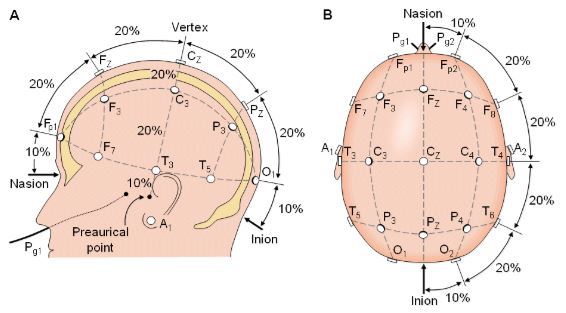
\includegraphics[scale=0.8]{{ImagesSSVEP/10_20}.jpg}}
  \captionsetup{singlelinecheck = false, justification=justified} % used for left alignment
  \caption{Τοποθεσίες ηλεκτροδίων με βάση το σύστημα 10-20.\\ Εικόνα από \cite{Malmivuo2012Bioelectromagnetism:Fields}. }
  \label{fig:10_20}
\end{figure}

Ανάλογα με την εγκεφαλική περιοχή που καλύπτουν τα ηλεκτρόδια, παίρνουν και το όνομά τους που αποτελείται από ένα γράμμα (η συνδυασμό γραμμάτων) και έναν ζυγό αριθμό για το δεξί ημισφαίριο και περιττό για το αριστερό ημισφαίριο. Η βασική διάταξη που αποτελείται από 19 ηλεκτρόδια, είναι η εξής :

\begin{itemize}
    \item Προμετωπιαίος φλοιός (Pre-Frontal cortex) : Fp1, Fp2
    \item Μετωπιαίος λοβός (Frontal lobe) : F3, F4, F7, F8, Fz
    \item Κροταφικός λοβός (Temporal lobe) : T3, T4, T5, T6
    \item Βρεγματικός λοβός (Parietal lobe) : P3, P4, Pz
    \item Ινιακός λοβός (Occipital lobe) : O1, O2
    \item Κεντρική περιοχή (Central) : C3, C4, Cz
\end{itemize}
\par Ο δείκτης z, προσδιορίζει τα ηλεκτρόδια τα οποία βρίσκονται πάνω στην διαχωριστική γραμμή μεταξύ των δύο ημισφαιρίων.
Το παραπάνω σύστημα μπορεί να επεκταθεί έτσι ώστε να καλύψει καταστάσεις στις οποίες απαιτείται μεγαλύτερος αριθμός ηλεκτροδίων, ορίζοντας νέες εγκεφαλικές περιοχές μεταξύ αυτών που αναφέρθηκαν, ή και διαφορετικές σχετικές αποστάσεις μεταξύ των ηλεκτροδίων.
\begin{figure}[h]
  \centering
  \noindent\makebox[\textwidth]{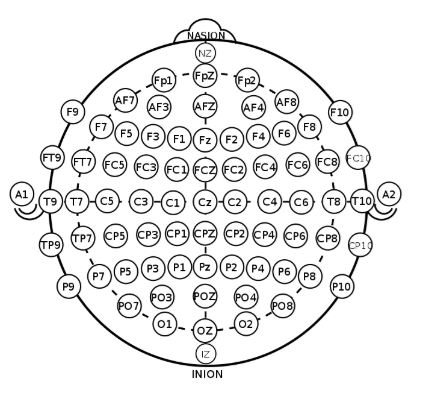
\includegraphics[scale=0.6]{{ImagesSSVEP/10_20_ext}.jpg}}
  \captionsetup{singlelinecheck = false, justification=justified} % used for left alignment
  \caption{Επέκταση συστήματος 10-20 .\\ Εικόνα από \cite{Malmivuo2012Bioelectromagnetism:Fields}. }
  \label{fig:10_20_ext}
\end{figure}

\end{document}
